\documentclass{article}
\usepackage{graphicx}
\begin{document}
\part{The Origin of Adrio Kusmareza Adim}
\section{Early Life}
The only memorable thing about December beside my ex and my sister birthday is the deadline for Kala December issue. Back in 2011, I was Kala Magazine editor-in-chief for the December issue and worked with nine fellow students from the journalism science department. \cite{einstein}

\begin{figure}[htb]
	\begin{center}
		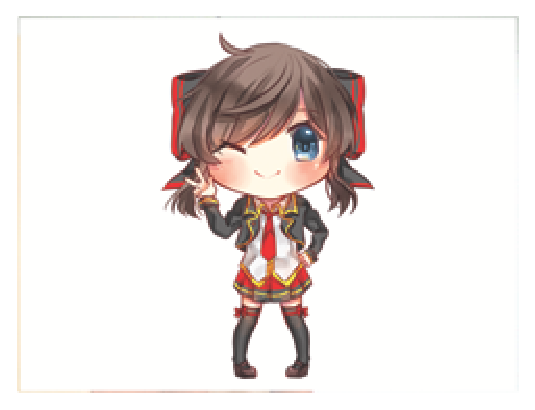
\includegraphics[width=6.0cm]{adrio.eps}
		\caption{Random Things}
		\label{fig:figure1}
	\end{center}
\end{figure}

\section{Today}
Kala Magazine is a digital magazine project for Printed Journalism Production course and also part of Bandung Citizen Magazine, a news portal which is ran by both students and faculty members from the journalism science at University of Padjadjaran. The goal of this joint project was a multimedia journalism experiment for students. \cite{latexcompanion}

\section{Future}
My class was divided into teams of ten and each team was responsible for an issue. In many classes here, lottery is always the answer for all team related problem. Many of my teachers here used this method to encourage students to engage in an unfamiliar topic. As a team leader, it is my job to play this game of luck with the other leaders. At the time, I did not know what month that myself or my team wanted, I prayed to God for the best. When picking up that white sushi rolled piece of paper, reality slapped me in the face. I was afraid that I drew a month so lame; my team would hunt me even in the afterlife. \cite{knuthwebsite}

\begin{table}[htb]
	\caption{Kawaii}
	\label{tab:kawaii}
\begin{center}
\begin{tabular}{||c|c|c||}
	\hline
No & Anime & Review \\
	\hline\hline
1 & Attack on Titan & Bad \\
	\hline
2 & Sword Art Online & OK \\
	\hline
3 & Re Zero & Emilia DAISUKI \\
	\hline
4 & Bakuon & OK \\
	\hline
\end{tabular}
\end{center}
\end{table}

\section{Encore}
Things that I Like So Much
\begin{itemize}
\item LoveLive
\item iDOLM@STTER
\item Hikari-chan from Digimon tri
\end{itemize}

\nocite{*}
\bibliographystyle{junsrt2}
\bibliography{mybib}

\end{document}